
\begin{dang}{Sự biến thiên của hàm số lượng giác}
\begin{itemize}
	\item Hàm số $y = \sin x$ đồng biến trên mỗi khoảng $\left(-\dfrac{\pi}{2}+k2\pi;\dfrac{\pi}{2}+k2\pi\right)$ $(k \in \mathbb{Z})$ và nghịch biến trên mỗi khoảng $\left(\dfrac{\pi}{2}+k2\pi;\dfrac{3\pi}{2}+k2\pi\right)$ $(k \in \mathbb{Z})$.\\
	% Ta có đồ thị của hàm số $y = \sin x$ trên $\mathbb{R}$ như sau
	% \begin{center}
	% 	\begin{tikzpicture}[scale=0.8,>=stealth, font=\footnotesize, line join=round, line cap=round]
	% 		\def\xmin{-10} \def\xmax{10.5} \def\ymin{-1.5} \def\ymax{1.8}
	% 		\draw[->] (\xmin,0)--(\xmax,0) node [below]{$x$};
	% 		\draw[->] (0,\ymin)--(0,\ymax) node [right]{$y$};
	% 		\node at (0,0) [below right]{$O$};
	% 		\clip (\xmin+0.1,\ymin+0.1) rectangle (\xmax-0.5,\ymax-0.1);
	% 		\draw[smooth,samples=400,domain=\xmin:\xmax] plot(\x,{sin(\x r)});
	% 		\draw[dashed] (\xmin,1)--(\xmax,1) (\xmin,-1)--(\xmax,-1);
	% 		\foreach \x in {-3*pi,-2.5*pi,-2*pi,-1.5*pi,-pi,-0.5*pi,0}
	% 		{\draw[fill=black] (\x,sin \x*180/pi) circle (1pt);
	% 			\draw[dashed] (\x,sin \x*180/pi)--(\x,0);
	% 			\draw[fill=black] (-\x,sin -\x*180/pi) circle (1pt);
	% 			\draw[dashed] (-\x,sin -\x*180/pi)--(-\x,0);}
	% 		\node at (0,1.3) [left]{$1$};
	% 		\node at (0,-1.3) [left]{$-1$};
	% 		\node at (-2*pi+0.15,0) [below]{$-2\pi$};
	% 		\node at (-3*pi-0.15,0) [below]{$-3\pi$};
	% 		\node at (-2.5*pi,0) [above]{$-\frac{5\pi}{2}$};
	% 		\node at (-1.5*pi,0) [below]{$-\frac{3\pi}{2}$};
	% 		\node at (-pi-0.15,0) [below]{$-\pi$};
	% 		\node at (-0.5*pi,0) [above]{$-\frac{\pi}{2}$};
	% 		\node at (0.5*pi,0) [below]{$\frac{\pi}{2}$};
	% 		\node at (pi-0.1,0) [below]{$\pi$};
	% 		\node at (1.5*pi,0) [above]{$\frac{3\pi}{2}$};
	% 		\node at (2*pi+0.2,0) [below]{$2\pi$};
	% 		\node at (2.5*pi+0.2,0) [below]{$\frac{5\pi}{2}$};
	% 		\node at (3*pi+0.2,0) [below]{$3\pi$};
	% 		\node at (2.5*pi+1,0.8) [above]{$y=\sin x$};
	% 	\end{tikzpicture}
	% \end{center}
	
	\item Hàm số $y = \cos x$ đồng biến trên mỗi khoảng $\left(-\pi+k2\pi; k2\pi\right)$ $(k \in \mathbb{Z})$ và nghịch biến trên mỗi khoảng $\left(k2\pi;\pi+k2\pi\right)$ $(k \in \mathbb{Z})$.\\
	% Ta có đồ thị của hàm số $y = \cos x$ trên $\mathbb{R}$ như sau
	% \begin{center}
	% 	\begin{tikzpicture}[scale=0.8,>=stealth, font=\footnotesize, line join=round, line cap=round]
	% 		\def\xmin{-10} \def\xmax{10.5} \def\ymin{-1.5} \def\ymax{1.8}
	% 		\draw[->] (\xmin,0)--(\xmax,0) node [below]{$x$};
	% 		\draw[->] (0,\ymin)--(0,\ymax) node [right]{$y$};
	% 		\node at (0,0) [below right]{$O$};
	% 		\clip (\xmin+0.1,\ymin+0.1) rectangle (\xmax-0.5,\ymax-0.1);
	% 		\draw[smooth,samples=400,domain=\xmin:\xmax] plot(\x,{cos(\x r)});
	% 		\draw[dashed] (\xmin,1)--(\xmax,1) (\xmin,-1)--(\xmax,-1);
	% 		\foreach \x in {-3*pi,-2.5*pi,-2*pi,-1.5*pi,-pi,-0.5*pi,0}
	% 		{\draw[fill=black] (\x,cos \x*180/pi) circle (1pt);
	% 			\draw[dashed] (\x,cos \x*180/pi)--(\x,0);
	% 			\draw[fill=black] (-\x,cos -\x*180/pi) circle (1pt);
	% 			\draw[dashed] (-\x,cos \x*180/pi)--(-\x,0);}
	% 		\node at (0,1.3) [left]{$1$};
	% 		\node at (0,-1.3) [left]{$-1$};
	% 		\node at (-2*pi+0.15,0) [below]{$-2\pi$};
	% 		\node at (-3*pi-0.15,0) [above]{$-3\pi$};
	% 		\node at (-2.5*pi,0) [above]{$-\frac{5\pi}{2}$};
	% 		\node at (-1.5*pi,0) [below]{$-\frac{3\pi}{2}$};
	% 		\node at (-pi-0.15,0) [above]{$-\pi$};
	% 		\node at (-0.5*pi,0) [above]{$-\frac{\pi}{2}$};
	% 		\node at (0.5*pi,0) [below]{$\frac{\pi}{2}$};
	% 		\node at (pi-0.1,0) [above]{$\pi$};
	% 		\node at (1.5*pi,0) [above]{$\frac{3\pi}{2}$};
	% 		\node at (2*pi+0.2,0) [below]{$2\pi$};
	% 		\node at (2.5*pi+0.2,0) [below]{$\frac{5\pi}{2}$};
	% 		\node at (3*pi+0.2,0) [above]{$3\pi$};
	% 		\node at (1.6*pi+1,0.8) [above]{$y=\cos x$};
	% 	\end{tikzpicture}
	% \end{center}
	
	\item Hàm số $y = \tan x$ đồng biến trên mỗi khoảng $\left(-\dfrac{\pi}{2}+k\pi;\dfrac{\pi}{2}+k\pi\right)$ $(k \in \mathbb{Z})$. 
	% \immini{	\textbf{Hàm số $y = \tan x$}\\
	% 	Ta có đồ thị của hàm số $y = \tan x$ trên $\mathbb{R}\setminus\left\{\dfrac{\pi}{2}+k\pi|k \in \mathbb{Z}\right\}$ như hình bên. Hàm số đồng biến trên mỗi khoảng $\left(-\dfrac{\pi}{2}+k\pi;\dfrac{\pi}{2}+k\pi\right)$ $(k \in \mathbb{Z})$. }{	\begin{tikzpicture}[scale=0.8,>=stealth, font=\footnotesize, line join=round, line cap=round]
	% 		\def\xmin{-5.5} \def\xmax{5.5} \def\ymin{-3} \def\ymax{3}
	% 		\draw[->] (\xmin,0)--(\xmax,0) node [below]{$x$};
	% 		\draw[->] (0,\ymin)--(0,\ymax) node [right]{$y$};
	% 		\node at (0,0) [below right]{$O$};
	% 		\clip (\xmin+0.1,\ymin+0.1) rectangle (\xmax-0.5,\ymax-0.1);
	% 		\draw[smooth,samples=400,domain=\xmin:\xmax] plot(\x,{tan(\x r)});
	% 		\node at (-2*pi-0.2,0) [above]{$-2\pi$};
	% 		\node at (-1.5*pi-0.4,0) [below]{$-\frac{3\pi}{2}$};
	% 		\node at (-pi-0.2,0) [above]{$-\pi$};
	% 		\node at (-0.5*pi-0.4,0) [below]{$-\frac{\pi}{2}$};
	% 		\node at (0.5*pi-0.2,0) [below]{$\frac{\pi}{2}$};
	% 		\node at (pi-0.1,0) [above]{$\pi$};
	% 		\node at (1.5*pi-0.3,0) [below]{$\frac{3\pi}{2}$};
	% 		\node at (2*pi+0.2,0) [below]{$2\pi$};
	% 		\node at (1.1*pi+0.2,2.7) [below]{$y = \tan x$};
	% \end{tikzpicture}}
	\item Hàm số $y = \cot x$ nghịch biến trên mỗi khoảng $\left(k\pi;\pi+k\pi\right)$ $(k \in \mathbb{Z})$. 
	% \immini{	\textbf{Hàm số $y = \cot x$}\\
	% 	Ta có đồ thị của hàm số $y = \cot x$ trên $\mathbb{R}\setminus\left\{k\pi|k \in \mathbb{Z}\right\}$ như hình bên.  Hàm số nghịch biến trên mỗi khoảng $\left(k\pi;\pi+k\pi\right)$ $(k \in \mathbb{Z})$. }{	\begin{tikzpicture}[scale=0.8,>=stealth, font=\footnotesize, line join=round, line cap=round]
	% 		\def\xmin{-7} \def\xmax{6.5} \def\ymin{-4} \def\ymax{4}
	% 		\draw[->] (\xmin,0)--(\xmax,0) node [below]{$x$};
	% 		\draw[->] (0,\ymin)--(0,\ymax) node [left]{$y$};
	% 		\node at (0,0) [above left]{$O$};
	% 		\clip (\xmin+0.1,\ymin+0.1) rectangle (\xmax-0.5,\ymax-0.1);
	% 		\foreach \n in {-2,-1,0,1}
	% 		{\draw[smooth,samples=400,domain=(\n+0.05)*pi:(\n+0.95)*pi] plot(\x,{1/tan(\x r)});
	% 			\draw (\n*pi,\ymin)--(\n*pi,\ymax);}
	% 		\node at (-2*pi-0.4,0) [below]{$-2\pi$};
	% 		\node at (-1.5*pi-0.3,0) [below]{$-\frac{3\pi}{2}$};
	% 		\node at (-pi-0.3,0) [below]{$-\pi$};
	% 		\node at (-0.5*pi-0.3,0) [below]{$-\frac{\pi}{2}$};
	% 		\node at (0.5*pi-0.1,0) [below]{$\frac{\pi}{2}$};
	% 		\node at (pi-0.2,0) [below]{$\pi$};
	% 		\node at (1.5*pi-0.2,0) [below]{$\frac{3\pi}{2}$};
	% 		\node at (1.5*pi-0.2,2.5) [above]{$y=\cot x$};
	% \end{tikzpicture}}
\end{itemize}
\end{dang}
%\setcounter{ex}{0}
\viduminhhoa

\begin{vd} Xét sự biến thiên của mỗi hàm số sau trên các khoảng tương ứng:
	\begin{enumerate}[a)]
		\item 	$y=\sin x$ trên khoảng $\left(-\dfrac{9 \pi}{2} ;-\dfrac{7 \pi}{2}\right),\left(\dfrac{21 \pi}{2} ; \dfrac{23 \pi}{2}\right)$;
		\item 	$y=\cos x$ trên khoảng $(-20 \pi ;-19 \pi),(-9 \pi ;-8 \pi)$.
	\end{enumerate}
	\loigiai{
		\hfill
		\begin{enumerate}[a)]
			\item Ta có
			\begin{itemize}
				\item $\left( -\dfrac{9\pi }{2};-\dfrac{7\pi }{2} \right)=\,\left( -\dfrac{\pi }{2}-4\pi ;\dfrac{\pi }{2}-4\pi  \right)$.\\
				Do hàm số $y=\sin x$ đồng biến trên khoảng $\left(-\dfrac{\pi}{2};\dfrac{\pi}{2}\right)$ nên hàm số đó cũng đồng biến trên khoảng $\left(-\dfrac{9\pi}{2};-\dfrac{7\pi}{2}\right)$.
				\item $\left( \dfrac{21\pi }{2};\dfrac{23\pi }{2} \right)=\left( \dfrac{\pi }{2}+10\pi ;\dfrac{3\pi }{2}+10\pi  \right)$.\\
				Do hàm số $y=\sin x$ nghịch biến trên khoảng $\left(\dfrac{\pi}{2};\dfrac{3\pi}{2}\right)$ nên hàm số đó cũng nghịch biến trên khoảng $\left(\dfrac{21\pi}{2};\dfrac{23\pi}{2}\right)$ .
			\end{itemize}
			\item Ta có
			\begin{itemize}
				\item $\left( -20\pi ;-19\pi  \right)=\left( 0-20\pi ;\pi -20\pi  \right)$.\\
				Do hàm số $y=\cos x$ nghịch biến trên khoảng $\left(0;\pi\right)$ nên hàm số đó cũng nghịch biến trên khoảng $\left(-20\pi ;-19\pi\right)$
				\item $\left( -9\pi ;-8\pi  \right)=\left( -\pi -8\pi ;0-8\pi  \right)$.\\
				Do hàm số $y=\cos x$ đồng biến trên khoảng $\left(-\pi ;0\right)$ nên hàm số đó cũng đồng biến trên khoảng $\left(-9\pi ;-8\pi\right)$
			\end{itemize}
		\end{enumerate}
	}
\end{vd}
\dongcham{8}
\begin{vd} Một dao động điều hoà có phương trình li độ dao động là: $x=A\cos\left(\omega\,t+\varphi\right)$ , trong đó $t$ là thời gian tính bằng giây, $A$ là biên độ dao động và $x$ là li độ dao động đều được tính bằng centimét, $\omega >0$ . Khi đó, chu kì $T$ của dao động là $T=\dfrac{2\pi}{\omega}$ . Xác định giá trị của li độ khi $t=0,\,\,t=\dfrac{T}{4},\,\,t=\dfrac{T}{2},\,t=\dfrac{3T}{4},\,\,t=T$ và vẽ đồ thị biểu diễn li độ của dao động điều hoà trên đoạn $\left[0;2T\right]$ trong các trường hợp:
	\begin{tasks}(3)
		\task $A=3cm,\,\,\varphi=0$;
		\task $A=3cm,\,\,\varphi=-\dfrac{\pi}{2}$;
		\task $A=3cm,\,\,\varphi=\dfrac{\pi}{2}$.
	\end{tasks}
	\loigiai{
		%		\begin{figure}
			\begin{enumerate}[a)]
				\item Khi $A=3cm,\,\,\varphi=0$, ta có: $x=3\cos\left(\omega\,t\right)=3\cos\left(\dfrac{2\pi}{T}t\right)$.\\
				\immini
				{Ta có bảng xác định giá trị li độ tại một số thời điểm và đồ thị cần vẽ ở Hình 9:\\
					\begin{tabular}{|c|c|c|c|c|c|}
						\hline
						$t$ &$0$  &$\dfrac{T}{4}$  &$\dfrac{T}{2}$  &$\dfrac{3T}{4}$  &$T$  \\
						\hline
						$x$ &$3$  &$0$  &$-3$  &$0$  &$3$  \\
						\hline
					\end{tabular}
				}{
					\begin{tikzpicture} [scale=0.6,>=stealth, font=\footnotesize, line join=round, line cap=round]
						\draw[->] (0,0)--(4*pi+0.5,0) node[above] {$t$};
						\draw[->] (0,-3.5)--(0,3.5) node[below left]{$x$};
						\draw (0,0) node[below left]{$O$};
						\def\xmin{0} \def\xmax{4*pi}
						\draw[domain=\xmin:\xmax,samples=100, smooth] plot (\x, {3*cos(\x r)});
						\draw[dashed] (\xmin,3)--(\xmax+0.5,3) (\xmin,-3)--(\xmax+0.5,-3);
						\node at (0.5*pi,0) [below left]{$\dfrac{T}{4}$};
						\node at (pi,0) [above]{$\dfrac{T}{2}$};
						\node at (1.5*pi,0) [below right]{$\dfrac{3T}{4}$};
						\node at (2*pi,0) [below]{$T$};
						\node at (2.5*pi,0) [below left]{$\dfrac{5T}{4}$};
						\node at (3*pi,0) [above]{$\dfrac{3T}{2}$};
						\node at (3.5*pi,0) [below right]{$\dfrac{7T}{4}$};
						\node at (4*pi,0) [below]{$2T$};
						\draw[dashed] (pi,0)--(pi,-3);
						\draw[dashed] (2*pi,0)--(2*pi,3);
						\draw[dashed] (3*pi,0)--(3*pi,-3);
						\draw[dashed] (4*pi,0)--(4*pi,3);
					\end{tikzpicture}
					%			\caption{}
				}
				\item Khi $A=3cm,\,\,\varphi=-\dfrac{\pi}{2}$, ta có: $x=3\cos\left(\omega\,t-\dfrac{\pi}{2}\right)=3\cos\left(\dfrac{2\pi}{T}t-\dfrac{\pi}{2}\right)$.
				\immini
				{Ta có bảng xác định giá trị li độ tại một số thời điểm và đồ thị cần vẽ ở Hình 10:\\
					\begin{tabular}{|c|c|c|c|c|c|}
						\hline
						$t$ &$0$  &$\dfrac{T}{4}$  &$\dfrac{T}{2}$  &$\dfrac{3T}{4}$  &$T$  \\
						\hline
						$x$ &$0$  &$3$  &$0$  &$-3$    &$0$  \\
						\hline
					\end{tabular}
				}
				{
					\begin{tikzpicture} [scale=0.6,>=stealth, font=\footnotesize, line join=round, line cap=round]
						\draw[->] (0,0)--(4*pi+0.5,0) node[above] {$t$};
						\draw[->] (0,-3.5)--(0,3.5) node[below left]{$x$};
						\draw (0,0) node[below left]{$O$};
						\def\xmin{0} \def\xmax{4*pi}
						\draw[domain=\xmin:\xmax,samples=100, smooth] plot (\x, {3*cos((\x-0.5*pi) r)});
						\draw[dashed] (\xmin,3)--(\xmax+0.5,3) (\xmin,-3)--(\xmax+0.5,-3);
						\node at (0.5*pi,0) [below left]{$\dfrac{T}{4}$};
						\node at (pi,0) [below left]{$\dfrac{T}{2}$};
						\node at (1.5*pi,0) [above]{$\dfrac{3T}{4}$};
						\node at (2*pi,0) [below right]{$T$};
						\node at (2.5*pi,0) [below]{$\dfrac{5T}{4}$};
						\node at (3*pi,0) [below left]{$\dfrac{3T}{2}$};
						\node at (3.5*pi,0) [above]{$\dfrac{7T}{4}$};
						\node at (4*pi,0) [below right]{$2T$};
						\draw[dashed] (0.5*pi,0)--(0.5*pi,3);
						\draw[dashed] (1.5*pi,0)--(1.5*pi,-3);
						\draw[dashed] (2.5*pi,0)--(2.5*pi,3);
						\draw[dashed] (3.5*pi,0)--(3.5*pi,-3);
					\end{tikzpicture}
					%			\caption{}
				}
				\item Khi $A=3cm,\,\,\varphi=\dfrac{\pi}{2}$, ta có: $x=3\cos\left(\omega\,t+\dfrac{\pi}{2}\right)=3\cos\left(\dfrac{2\pi}{T}t+\dfrac{\pi}{2}\right)$.
				\immini
				{Ta có bảng xác định giá trị li độ tại một số thời điểm và đồ thị cần vẽ ở Hình 11:\\
					\begin{tabular}{|c|c|c|c|c|c|}
						\hline
						$t$ &$0$  &$\dfrac{T}{4}$  &$\dfrac{T}{2}$  &$\dfrac{3T}{4}$  &$T$  \\
						\hline
						$x$ &$0$  &$-3$  &$0$  &$3$    &$0$  \\
						\hline
					\end{tabular}
				}
				{
					\begin{tikzpicture} [scale=0.6,>=stealth, font=\footnotesize, line join=round, line cap=round]
						\draw[->] (0,0)--(4*pi+0.5,0) node[above] {$t$};
						\draw[->] (0,-3.5)--(0,3.5) node[below left]{$x$};
						\draw (0,0) node[below left]{$O$};
						\def\xmin{0} \def\xmax{4*pi}
						\draw[domain=\xmin:\xmax,samples=100, smooth] plot (\x, {3*cos((\x+0.5*pi) r)});
						\draw[dashed] (\xmin,3)--(\xmax+0.5,3) (\xmin,-3)--(\xmax+0.5,-3);
						\node at (0.5*pi,0) [above]{$\dfrac{T}{4}$};
						\node at (pi,0) [below right]{$\dfrac{T}{2}$};
						\node at (1.5*pi,0) [below]{$\dfrac{3T}{4}$};
						\node at (2*pi,0) [below left]{$T$};
						\node at (2.5*pi,0) [above]{$\dfrac{5T}{4}$};
						\node at (3*pi,0) [below right]{$\dfrac{3T}{2}$};
						\node at (3.5*pi,0) [below]{$\dfrac{7T}{4}$};
						\node at (4*pi,0) [below]{$2T$};
						\draw[dashed] (0.5*pi,0)--(0.5*pi,-3);
						\draw[dashed] (1.5*pi,0)--(1.5*pi,3);
						\draw[dashed] (2.5*pi,0)--(2.5*pi,-3);
						\draw[dashed] (3.5*pi,0)--(3.5*pi,3);
					\end{tikzpicture}
					%			\caption{}
				}
			\end{enumerate}
			%	\end{figure}
	}
\end{vd}
\baitaptn
\Opensolutionfile{ans}[ans/ans-1K1-3-dang5]
\begin{ex}%[1D1B1-2]%Câu 1.
	Hàm số $y=\sin x$
	\choice
	{đồng biến trên mỗi khoảng $\left(\dfrac{\pi}{2}+k2\pi;\pi+k2\pi\right)$ và nghịch biến trên mỗi khoảng $\left(\pi+k2\pi;k2\pi\right)$ với $k\in\mathbb{Z}$}
	{đồng biến trên mỗi khoảng $\left(-\dfrac{3\pi}{2}+k2\pi;\dfrac{5\pi}{2}+k2\pi\right)$ và nghịch biến trên mỗi khoảng $\left(-\dfrac{\pi}{2}+k2\pi;\dfrac{\pi}{2}+k2\pi\right)$ với $k\in\mathbb{Z}$}
	{đồng biến trên mỗi khoảng $\left(\dfrac{\pi}{2}+k2\pi;\dfrac{3\pi}{2}+k2\pi\right)$ và nghịch biến trên mỗi khoảng $\left(-\dfrac{\pi}{2}+k2\pi;\dfrac{\pi}{2}+k2\pi\right)$ với $k\in\mathbb{Z}$}
	{\True đồng biến trên mỗi khoảng $\left(-\dfrac{\pi}{2}+k2\pi;\dfrac{\pi}{2}+k2\pi\right)$ và nghịch biến trên mỗi khoảng $\left(\dfrac{\pi}{2}+k2\pi;\dfrac{3\pi}{2}+k2\pi\right)$ với $k\in\mathbb{Z}$}
	\loigiai{
		\immini{
			Hàm số $y=\sin x$ đồng biến trên mỗi khoảng $\left(-\dfrac{\pi}{2}+k2\pi;\dfrac{\pi}{2}+k2\pi\right)$ và nghịch biến trên mỗi khoảng $\left(\dfrac{\pi}{2}+k2\pi;\dfrac{3\pi}{2}+k2\pi\right)$ với $k\in\mathbb{Z}$.}{
			\begin{tikzpicture}[scale=.7, font=\footnotesize, line join=round, line cap=round, >=stealth]
				% nhập vào hàm số
				\def\r{3} \def\m{3.5}
				\def\f(#1){(#1)}
				\draw[->] (-\r,0)--(\r+0.5,0) node[below] { $x$}node[above] { $\cos x$};
				\draw[->] (0,-\r)--(0,\r+0.5) node[below right] { $y$} node[left]{$\sin x$};
				\draw (0,0) node [below left] {$O$};
				\foreach \x/\g/\z in {2.5/-45/1,-2.5/-135/-1}\fill[black] (\x,0) circle (1pt)+(\g:0.4) node{$\z$};
				\foreach \y/\g/\z in {2.5/135/1,-2.5/-135/-1}\fill[black] (0,\y) circle (1pt)+(\g:0.4) node{$\z$};
				\draw[color=white] (0,0) circle (\r);
				\draw[-latex] (10:\r) arc (10:70:\r);
				\draw  (2.2,-0.2) node{$2\pi$}(2.3,0.2) node{$0$}(.2,2.1) node{$\tfrac{\pi}{2}$}(-.2,-2.1) node{$\tfrac{3\pi}{2}$}(-2.3,0.2) node{$\pi$};
				\draw[-latex] (-10:\r) arc (-10:-70:\r);
				\draw (0,0) circle (2.5);
				\draw (2,3)circle (6pt) node{$+$} (2,-3)circle (6pt) node{$-$};
			\end{tikzpicture}	
	}}
\end{ex}
\begin{ex}%[1D1B1-2]%Câu 2.
	Hàm số $y=\cos x$
	\choice
	{đồng biến trên mỗi khoảng $\left(\dfrac{\pi}{2}+k2\pi;\pi+k2\pi\right)$ và nghịch biến trên mỗi khoảng $\left(\pi+k2\pi;k2\pi\right)$ với $k\in\mathbb{Z}$}
	{\True đồng biến trên mỗi khoảng $\left(-\pi+k2\pi;k2\pi\right)$ và nghịch biến trên mỗi khoảng $\left(k2\pi;\pi+k2\pi\right)$ với $k\in\mathbb{Z}$}
	{đồng biến trên mỗi khoảng $\left(\dfrac{\pi}{2}+k2\pi;\dfrac{3\pi}{2}+k2\pi\right)$ và nghịch biến trên mỗi khoảng $\left(-\dfrac{\pi}{2}+k2\pi;\dfrac{\pi}{2}+k2\pi\right)$ với $k\in\mathbb{Z}$}
	{đồng biến trên mỗi khoảng $\left(k2\pi;\pi+k2\pi\right)$ và nghịch biến trên mỗi khoảng $\left(\pi+k2\pi;3\pi+k2\pi\right)$ với $k\in\mathbb{Z}$}
	\loigiai{
		\immini{
			Hàm số $y=\cos x$ đồng biến trên mỗi khoảng $\left(-\pi+k2\pi;k2\pi\right)$ và nghịch biến trên mỗi khoảng $\left(k2\pi;\pi+k2\pi\right)$ với $k\in\mathbb{Z}$.}
		{
			\begin{tikzpicture}[scale=.7, font=\footnotesize, line join=round, line cap=round, >=stealth]
				% nhập vào hàm số
				\def\r{3} \def\m{3.5}
				\def\f(#1){(#1)}
				\draw[->] (-\r,0)--(\r+0.5,0) node[below] { $x$}node[above] { $\cos x$};
				\draw[->] (0,-\r)--(0,\r+0.5) node[below right] { $y$} node[left]{$\sin x$};
				\draw (0,0) node [below left] {$O$};
				\foreach \x/\g/\z in {2.5/-45/1,-2.5/-135/-1}\fill[black] (\x,0) circle (1pt)+(\g:0.4) node{$\z$};
				\foreach \y/\g/\z in {2.5/135/1,-2.5/-135/-1}\fill[black] (0,\y) circle (1pt)+(\g:0.4) node{$\z$};
				\draw[color=white] (0,0) circle (\r);
				\draw[-latex] (10:\r) arc (10:70:\r);
				\draw  (2.2,-0.2) node{$2\pi$}(2.3,0.2) node{$0$}(.2,2.1) node{$\tfrac{\pi}{2}$}(-.2,-2.1) node{$\tfrac{3\pi}{2}$}(-2.3,0.2) node{$\pi$};
				\draw[-latex] (-10:\r) arc (-10:-70:\r);
				\draw (0,0) circle (2.5);
				\draw (2,3)circle (6pt) node{$+$} (2,-3)circle (6pt) node{$-$};
			\end{tikzpicture}	
	}}
\end{ex}
\begin{ex}%[1D1B1-2]
	Hàm số $y=\tan x$ đồng biến trên khoảng nào sau đây?
	\choice{\True $\left(0;\dfrac{\pi}{2}\right)$}{$(0;\pi)$}{$\left(\dfrac{\pi}{2};2 \pi\right)$}{$\left(\dfrac{\pi}{2};\dfrac{5 \pi}{2}\right)$}
	\loigiai{
		Hàm số $y=\tan x$ luôn đồng biến trên các khoảng xác định, vậy nó đồng biến trên khoảng $\left(0;\dfrac{\pi}{2}\right)$.
	}
\end{ex}
\begin{ex}%[1D1B1-2]
	Hàm số $y= \cot x$ nghịch biến trên khoảng nào sau đây?
	\choice{$(0;2\pi)$}{$\left(\dfrac{\pi}{2};2 \pi\right)$}{\True $(-\pi;0)$}{$\left(\dfrac{\pi}{2};\dfrac{3 \pi}{2}\right)$}
	\loigiai{
		Hàm số $y=\cot x$ luôn nghịch biến trên các khoảng xác định.\\
		Vậy hàm số nghịch biến trên khoảng $(0;\pi)$.
	}
\end{ex}
\begin{ex}%[1D1B1-2]%Câu 3.
	Hàm số $y=\sqrt{3}+2\cos x$ tăng trên khoảng
	\choice
	{$\left(-\dfrac{\pi}{6};\dfrac{\pi}{2}\right)$}
	{$\left(\dfrac{\pi}{2};\dfrac{3\pi}{2}\right)$}
	{\True $\left(\dfrac{7\pi}{6};2\pi\right)$}
	{$\left(\dfrac{\pi}{6};\dfrac{\pi}{2}\right)$}
	\loigiai{
		\immini{
			Vì hàm số $y=\cos x$ đồng biến trên mỗi khoảng $\left(-\pi+k2\pi;k2\pi\right)$, $k\in\mathbb{Z}$ nên hàm số $y=\sqrt{3}+2\cos x$ cũng đồng biến trên mỗi khoảng $\left(-\pi+k2\pi;k2\pi\right)$, $k\in\mathbb{Z}$.\\
			Vì $\left(\dfrac{7\pi}{6};2\pi\right)\subset(\pi;2\pi)$ (với $k=1$) nên hàm số đồng biến trên khoảng $\left(\dfrac{7\pi}{6};2\pi\right)$.}
		{
			\begin{tikzpicture}[scale=.7, font=\footnotesize, line join=round, line cap=round, >=stealth]
				% nhập vào hàm số
				\def\r{3} \def\m{3.5}
				\def\f(#1){(#1)}
				\draw[->] (-\r,0)--(\r+0.5,0) node[below] { $x$}node[above] { $\cos x$};
				\draw[->] (0,-\r)--(0,\r+0.5) node[below right] { $y$} node[left]{$\sin x$};
				\draw (0,0) node [below left] {$O$};
				\foreach \x/\g/\z in {2.5/-45/1,-2.5/-135/-1}\fill[black] (\x,0) circle (1pt)+(\g:0.4) node{$\z$};
				\foreach \y/\g/\z in {2.5/135/1,-2.5/-135/-1}\fill[black] (0,\y) circle (1pt)+(\g:0.4) node{$\z$};
				\draw[color=white] (0,0) circle (\r);
				\draw[-latex] (10:\r) arc (10:70:\r);
				\draw  (2.2,-0.2) node{$2\pi$}(2.3,0.2) node{$0$}(.2,2.1) node{$\tfrac{\pi}{2}$}(-.2,-2.1) node{$\tfrac{3\pi}{2}$}(-2.3,0.2) node{$\pi$};
				\draw[-latex] (-10:\r) arc (-10:-70:\r);
				\draw (0,0) circle (2.5);
				\draw (2,3)circle (6pt) node{$+$} (2,-3)circle (6pt) node{$-$};
			\end{tikzpicture}	
		}	
		
	}
\end{ex}
\begin{ex}%[1D1B1-2]%Câu 4.
	Hàm số nào đồng biến trên khoảng $\left(-\dfrac{\pi}{3};\dfrac{\pi}{6}\right)$?
	\choice
	{$y=\cos x$}
	{$y=\cot 2x$}
	{\True $y=\sin x$}
	{$y=\cos2x$}
	\loigiai{
		\immini{		
			Quan sát trên đường tròn lượng giác,
			ta thấy trên khoảng $\left(-\dfrac{\pi}{3};\dfrac{\pi}{6}\right)$ hàm số $y=\sin x$ tăng dần
			(tăng từ $-\dfrac{\sqrt{3}}{2}$ đến $\dfrac{1}{2}$).}
		{
			\begin{tikzpicture}[scale=.7, font=\footnotesize, line join=round, line cap=round, >=stealth]
				% nhập vào hàm số
				\def\r{3} \def\m{3.5}
				\def\f(#1){(#1)}
				\draw[->] (-\r,0)--(\r+0.5,0) node[below] { $x$}node[above] { $\cos x$};
				\draw[->] (0,-\r)--(0,\r+0.5) node[below right] { $y$} node[left]{$\sin x$};
				\draw (0,0) node [below left] {$O$};
				\draw [] (0,-2.25)--(1,-2.25)--(0,0)--(2.2,1.2)--(0,1.2);
				\foreach \x/\g/\z in {2.5/-45/1,-2.5/-135/-1}\fill[black] (\x,0) circle (1pt)+(\g:0.4) node{$\z$};
				\foreach \y/\g/\z in {2.5/135/1,-2.5/-135/-1}\fill[black] (0,\y) circle (1pt)+(\g:0.4) node{$\z$};
				\draw[color=white] (0,0) circle (\r);
				\draw[-latex] (10:\r) arc (10:70:\r);
				\draw[color=red] (0,-2.25)--(0,1.2); 
				\draw  (2.2,-0.2) node{$2\pi$}(2.3,0.2) node{$0$}(.2,2.1) node{$\tfrac{\pi}{2}$}(-.2,-2.1) node{$\tfrac{3\pi}{2}$}(-2.3,0.2) node{$\pi$} (2.5,1.2) node{$\tfrac{\pi}{6}$} (.75,-2.8) node{$-\tfrac{\pi}{3}$};
				\draw[-latex] (-10:\r) arc (-10:-70:\r);
				\draw (0,0) circle (2.5);
				\draw (2,3)circle (6pt) node{$+$} (2,-3)circle (6pt) node{$-$};
			\end{tikzpicture}	
		}	
	}
\end{ex}
% \begin{ex}%[1D1B1-2]%Câu 5.
% 	Mệnh đề nào sau đây \textbf{sai}?
% 	\choice
% 	{Hàm số $y=\sin x$ tăng trong khoảng $\left(0;\dfrac{\pi}{2}\right)$}
% 	{\True Hàm số $y=\cot x$ giảm trong khoảng $\left(0;\dfrac{\pi}{2}\right)$}
% 	{Hàm số $y=\tan x$ tăng trong khoảng $\left(0;\dfrac{\pi}{2}\right)$
% 	}
% 	{Hàm số $y=\cos x$ tăng trong khoảng $\left(0;\dfrac{\pi}{2}\right)$}
% 	\loigiai{
% 		\immini{
% 			Quan sát trên đường tròn lượng giác,
% 			trên khoảng $\left(0;\dfrac{\pi}{2}\right)$ ta thấy hàm số $y=\cos x$ giảm dần.}
% 		{
% 			\begin{tikzpicture}[scale=.7, font=\footnotesize, line join=round, line cap=round, >=stealth]
% 				% nhập vào hàm số
% 				\def\r{3} \def\m{3.5}
% 				\def\f(#1){(#1)}
% 				\draw[->] (-\r,0)--(\r+0.5,0) node[below] { $x$}node[above] { $\cos x$};
% 				\draw[->] (0,-\r)--(0,\r+0.5) node[below right] { $y$} node[left]{$\sin x$};
% 				\draw (0,0) node [below left] {$O$};
% 				\foreach \x/\g/\z in {2.5/-45/1,-2.5/-135/-1}\fill[black] (\x,0) circle (1pt)+(\g:0.4) node{$\z$};
% 				\foreach \y/\g/\z in {2.5/135/1,-2.5/-135/-1}\fill[black] (0,\y) circle (1pt)+(\g:0.4) node{$\z$};
% 				\draw[color=white] (0,0) circle (\r);
% 				\draw[-latex] (10:\r) arc (10:70:\r);
% 				\draw  (2.2,-0.2) node{$2\pi$}(2.3,0.2) node{$0$}(.2,2.1) node{$\tfrac{\pi}{2}$}(-.2,-2.1) node{$\tfrac{3\pi}{2}$}(-2.3,0.2) node{$\pi$};
% 				\draw[-latex] (-10:\r) arc (-10:-70:\r);
% 				\draw (0,0) circle (2.5);
% 				\draw[color=red] (0,0)--(2.5,0);
% 				\draw (2,3)circle (6pt) node{$+$} (2,-3)circle (6pt) node{$-$};
% 	\end{tikzpicture}}}
% \end{ex}
% \begin{ex}%[1D1B1-2]%Câu 7.
% 	Hàm số $y=\sin x$ đồng biến trên 
% 	\choice
% 	{khoảng $(0;\pi)$}
% 	{\True các khoảng $\left(-\dfrac{\pi}{4}+k2\pi;\dfrac{\pi}{4}+k2\pi\right)$, $k\in\mathbb{Z}$}
% 	{các khoảng $\left(\dfrac{\pi}{2}+k2\pi;\pi+k2\pi\right)$, $k\in\mathbb{Z}$}
% 	{khoảng $\left(\dfrac{\pi}{2};\dfrac{3\pi}{2}\right)$}
% 	\loigiai{
% 		Hàm số $y=\sin x$ đồng biến trên mỗi khoảng $\left(-\dfrac{\pi}{2}+k2\pi;\dfrac{\pi}{2}+k2\pi\right)$, $k\in\mathbb{Z}$.\\
% 		Mà $\left(-\dfrac{\pi}{4}+k2\pi;\dfrac{\pi}{4}+k2\pi\right)\subset\left(-\dfrac{\pi}{2}+k2\pi;\dfrac{\pi}{2}+k2\pi\right)$ với mỗi $k\in\mathbb{Z}$ nên hàm số đồng biến trên mỗi khoảng $\left(-\dfrac{\pi}{4}+k2\pi;\dfrac{\pi}{4}+k2\pi\right)$, $k\in\mathbb{Z}$.}
% \end{ex}

\Closesolutionfile{ans}
%\begin{indapan}{10}
%	{ans/ans-1K1-3-Dang2}
%\end{indapan}